\subsection{Assigning reviewers}

One of the primary reasons for using GitHub pull requests is to use its code review features.
We want both students and teachers to review code, with teachers explicitly having to approve a pull request for the assignment as a whole to be approved.

When assigning students we must make sure that no student is set to review an assignment they themselves have not yet completed.
Otherwise, we get a similar situation to the one mentioned in the previous challenge, where students have the option of plagiarising other students code.
Any implementation will have to make sure that students reviewing code should only review code they have already implemented.
A natural approach to this could be to have students only review code when the assignment deadline is passed.
At this point all students have gotten either a passing or failing grade, and QuickFeed can safely assign reviewers.

% No incentive for students to actually do code review when there is no penalty to refuse.

\subsection{Student feedback}

Another important feature is to have students receive automatic feedback on the code they write.
We envision that this feedback should come in the form of a score or grade, determined by tests run on the student's code.
Just as students currently receive feedback on an assignment as a whole, we want QuickFeed to do the same for tasks.

Currently, QuickFeed is only built around running tests on an assignment as a whole on the main branch.
To accommodate pull requests, QuickFeed would first need to be expanded so that it can run tests on other branches.
Secondly, QuickFeed will need the ability to run tests solely based on tasks.
The first accommodation is pretty straight forward, but the second one would require a rethink on how QuickFeed should approach the testing of code.

\subsection{Human Error}
% TODO: Can discuss these specifically in implementation part
Finally, we have to take into consideration the possibility that students may do things that we simply have not accounted for.

For example, they might delete issues that QuickFeed creates.
QuickFeed will then need to somehow recreate that issue, and restore a working state.

We will also have to account for students closing and possibly merging pull requests that are not yet approved by a teacher.
If this happens, QuickFeed must have the capacity to restore a working state for the task/assignment.

\subsection{Increased Complexity}

Introducing pull requests to students can prove challenging in itself.
Even though pull requests are not exactly a challenging feature to learn and use, it can still prove time consuming for certain students.
Even more so if students are already struggling with how to use git.
Having to swap between branches, making commits to them, and also knowing how to manage and create pull requests, are all things students will have to familiar with.
More time and effort from the teaching staff may therefore have to be dedicated to assisting students with issues they may have.

This is not an issue that can be explicitly solved.
Every teacher will have to decide themselves if the benefits outweigh the increased complexity when using tasks and pull request with their assignments.

\section{QuickFeed Expansion}
%% TODO: Move the contents from here to implementation.
Having simplified our approach in the previous section, we continue by looking at how we must expand QuickFeed to accommodate it.

\subsection{Tasks and GitHub Issues}
\label{sec:tasks_and_github_issues}

As a start, QuickFeed needs to support task markdown files in the \textit{tests} repository.
These task files will follow the standard format: \textit{task-*.md}.

\begin{figure}[ht]
    \centering
    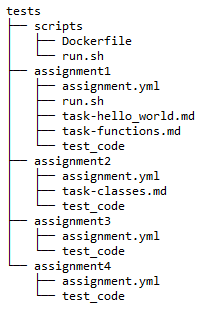
\includegraphics[scale=0.8]{photos/tests-repository-structure-tasks.PNG}
    \caption{Example of a tests repository with tasks}
    \label{fig:tests-repository-structure-tasks}
\end{figure}

As we see in the figure above, \textit{assignment1} and \textit{assignment2} both have tasks in them.

In essence we want these tasks to be represented as issues on all course group repositories.
This means that once a task is created by a teacher, and pushed to GitHub, the corresponding issues should be created on GitHub.
If a task is edited or deleted, QuickFeed must respectively either edit or delete the associated issue.
To manage the creation, deletion and editing of issues, QuickFeed's SCM API will be expanded to have such a capacity.

Beyond the ability to create, delete and edit issues, QuickFeed must be logically capable of determining when to perform these actions.
This means that QuickFeed will have to compare old tasks versus new ones, and then proceed accordingly.
We will therefore store representations of tasks in QuickFeed's internal database for this purpose.
Storing tasks also allows us to easily handle late enrolling groups, as we can use them to immediately create the required issues.

To edit issues, we will also need to internally store a reference to them in the database.

% To support pull requests, we need to expand

\section{Desired workflow}
% TODO: This part belongs in the introduction to the implementation chapter
This section describes in detail the desired student and teacher workflow, and is in essence what we want to achieve with this project.

Tasks will be handled as described in the previous section.
They are created by the teacher as markdown files within an assignment, and QuickFeed creates issues based on them.
When a student wants to complete any task, they create a new branch on their local repository.
Using this branch, they create a pull request on their student repository which is linked to the associated issue.

At this stage, a student has an open pull request on their repository.
Tests are run on the student code by QuickFeed, and students receive feedback on these tests in the pull request itself.

When students are finished with a task, i.e., they receive a passing score from the test results, their code is ready to be reviewed.
At this point, QuickFeed should automatically assign one student and teacher reviewer.
They will comment on the students code, request changes and so on.
When all changes are implemented, the teacher approves the pull request, allowing the student to merge it.
Finally, when all tasks have gone through this process, the assignment itself can be set as approved.

\section{Existing Approach}

An implementation for this project has already been attempted by Adil Khurshid. % TODO: Ref
This section discusses the approach he used.

In short, he proposed implementing support for the following features.
When a teacher creates an assignment, they have the option of creating any number of task markdown files.
For each of these markdown files, a single issue should be created on every student repository.
The title and body of these issues are defined by the contents of the corresponding task.
When a student wants to complete a task, they create a pull request for the associated issue.
After the deadline of the assignment has passed, QuickFeed randomly assigns co-student and teacher reviewers to the pull request. 
Only when the pull request has been approved by a teacher, should it be merged.

Adil discusses several challenges to this approach, and gives his proposed solutions.
Given that he did not finish his work however, many of these solutions have later proved inadequate or faulty, and in some cases potentially too complex.
In general, this thesis is independent of the aforementioned approach.

\subsection{Pull Requests}

The following questions are relevant for both this and the implementation part.

How do we listen to the webhook events that are relevant?
How do we single out the relevant events?
How should the pull requests be created?
How do we determine when to assign reviewers, when we do not have the ability to test based on tasks?
How do we ensure that reviewers are evenly distributed?
How do we ensure that reviewers are not assigned to their own repository?
What if a student pushes from a local branch that differs from a remote one?
What if an assignment is manually graded?
